\documentclass[a4paper]{article}

%% Language and font encodings
\usepackage[english]{babel}
\usepackage[utf8x]{inputenc}
\usepackage[T1]{fontenc}

%% Sets page size and margins
\usepackage[a4paper,top=3cm,bottom=2cm,left=3cm,right=3cm,marginparwidth=1.75cm]{geometry}

%% Useful packages
\usepackage{amsmath}
\usepackage{graphicx}
\usepackage[colorinlistoftodos]{todonotes}
\usepackage[colorlinks=true, allcolors=blue]{hyperref}

\title{Actividad 2}
\author{Isaac Neri Gómez Sarmiento}
\date{07 Febrero, 2018}
\begin{document}
\maketitle


\section{Introducción}

En esta actividad se hizo uso por primera vez del entorno de programación Jupyter Notebook, cuyo lenguaje principal de programación utilizado es Python. En combinación de las librerias de matplotlib, pandas y numpy, se hizo un análisis de datos obtenidos del Servicio Meteorológico Nacional del municipio de Iguala, Guerrero, México. 

\section{Desarrollo}
\subsection{Características y bondades}

Una de las características más llamativas, es que cada linea de código es ejecutada después de terminarla, sin necesidad de tenerla todas paras despues así poder ejecutarlo de una sola vez. Es de esperarse, pues Python es un lenguaje interpretado y no de compilación. Jupyter Notebook tiene la ventaja de poder visualizar en un mismo lugar, gráficas, tablas, imágenes, fórmulas, etc. sin salirse de la misma ventana.Aún mejor, permite también hacer uso de la sintaxis de latex para la creación de fórmulas y utilizar otros lenguajes de programación tales como R, Perl, Bash.

\subsection{Limitaciones y desventajas}
Posiblemente una limitación sería el tamaño de los archivos generados, ya que al tener tanto código como gráficas, tablas, imágenes, etc. su tamaño aumenta. A veces el código queda fragmentado,si no se sigue un orden, ya sea porque se hicieron varias pruebas de código en diferentes líneas y no salió el resultado esperado.

\subsection{Algunos comandos aprendidos}
Para ejecutar algún segmento de código se debe presionar las teclas "Shift y Enter" al mismo tiempo. 
Para poder manejar datos, usar expresiones matemáticas o graficar datos, se deben recurrir a librerias. 
Para leer archivos se recurre al comando "$pandas.read_csv$", donde csv lee datos con elementos separados por más de un espacio. 
Para poder ver el tipo de datos se utiliza el comando "$.dtypes$". Para realizar un análisis de datos se utiliza el comando .describe() después del nombre. En cuanto a las gráficas, para hacer una se debe primero usar el comando "plt.figure", y se le pueden agregar titulos con "plt.title". Aprendimos también a usar la herramienta ".describe", la cual hace un anális exploratorio de los datos, obteniendo datos como el promedio, desviación, min, max, etc. Finalmente se puedieron graficar los datos con el "comando plt.show()". 


\newpage
\subsection{Actividades a Realizar}
\textbf{1°Crear una gráfica que muestre la rapidez de los vientos y la rapidez de las ráfagas, como funciones del tiempo. ¿Cuáles son las horas del día con más viento?.}

\begin{figure}[ht!]
\centering
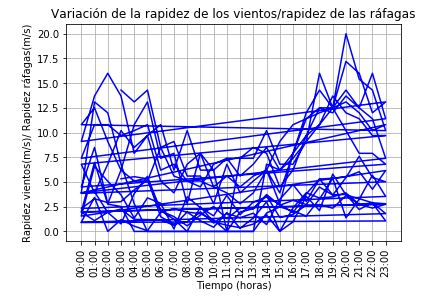
\includegraphics[width=0.5\textwidth]{Grafica_vientos_y_rafagas.JPG}
\caption{\label{fig:Vientos y rafagas }Vientos y rafagas}
\end{figure}

Esta gráfica representa las velocidades de los vientos y ráfagas en un intervalo de 7 días. En el eje de las x están las horas del dia y en el eje de las y se encuentran las velocidades. 
En la gráfica podemos apreciar que tanto en la madrugada como en la noche, se tienen los vientos más rápidos, mientras que en la mañana y medio dia se tienen los vientos más lentos.\\

\textbf{2° Crear una gráfica con la dirección de los vientos como función del tiempo y comentar sobre los vientos dominantes en el sitio de estudio.}

\begin{figure}[ht!]
\centering
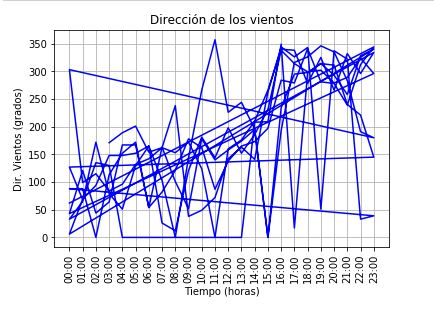
\includegraphics[width=0.5\textwidth]{Direcci_n_de_los_vientos.JPG}
\caption{\label{fig:Dirección de los vientos }Dirección de los vientos}
\end{figure}

En el eje de las x de esta gráfica están las horas del día y en el eje de las y se encuentra la dirección de los vientos en grados. A A pesar de ciertos comportamientos anómalos, se puede ver que la tendencia de los datos es que entre más avanza el día, la dirección de los vientos incrementa.\\

\newpage
\textbf{3° Muestre el comportamiento de la Radiación Solar como función del tiempo.¿Qué puedes comentar?} \\




\begin{figure}[ht!]
\centering
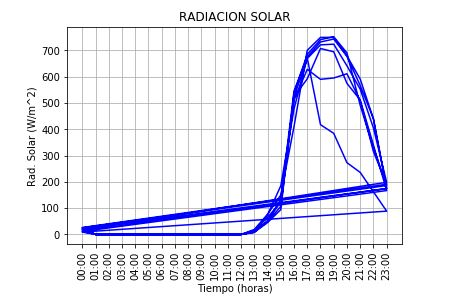
\includegraphics[width=0.5\textwidth]{Rad_Solar.JPG}
\caption{\label{fig:Radación Solar}Radiación Solar}
\end{figure}

En este gráfica, el \textit{eje x} representa las horas del día, mientras que el \textit{eje y} representa la radiación solar, cuyas unidades no estaban claras, así que se definieron como W/m$^2$. Si nos ponemos a analizar la gráfica, podemos notar algunas incongruencias, ya que muestra que la hora de mayor radiación solar es entre las 17 y 18 horas. Esto se debe a que la medición de las horas fueron respecto al huso horario del meridiano de Greenwich. 

\begin{figure}[ht!]
\centering
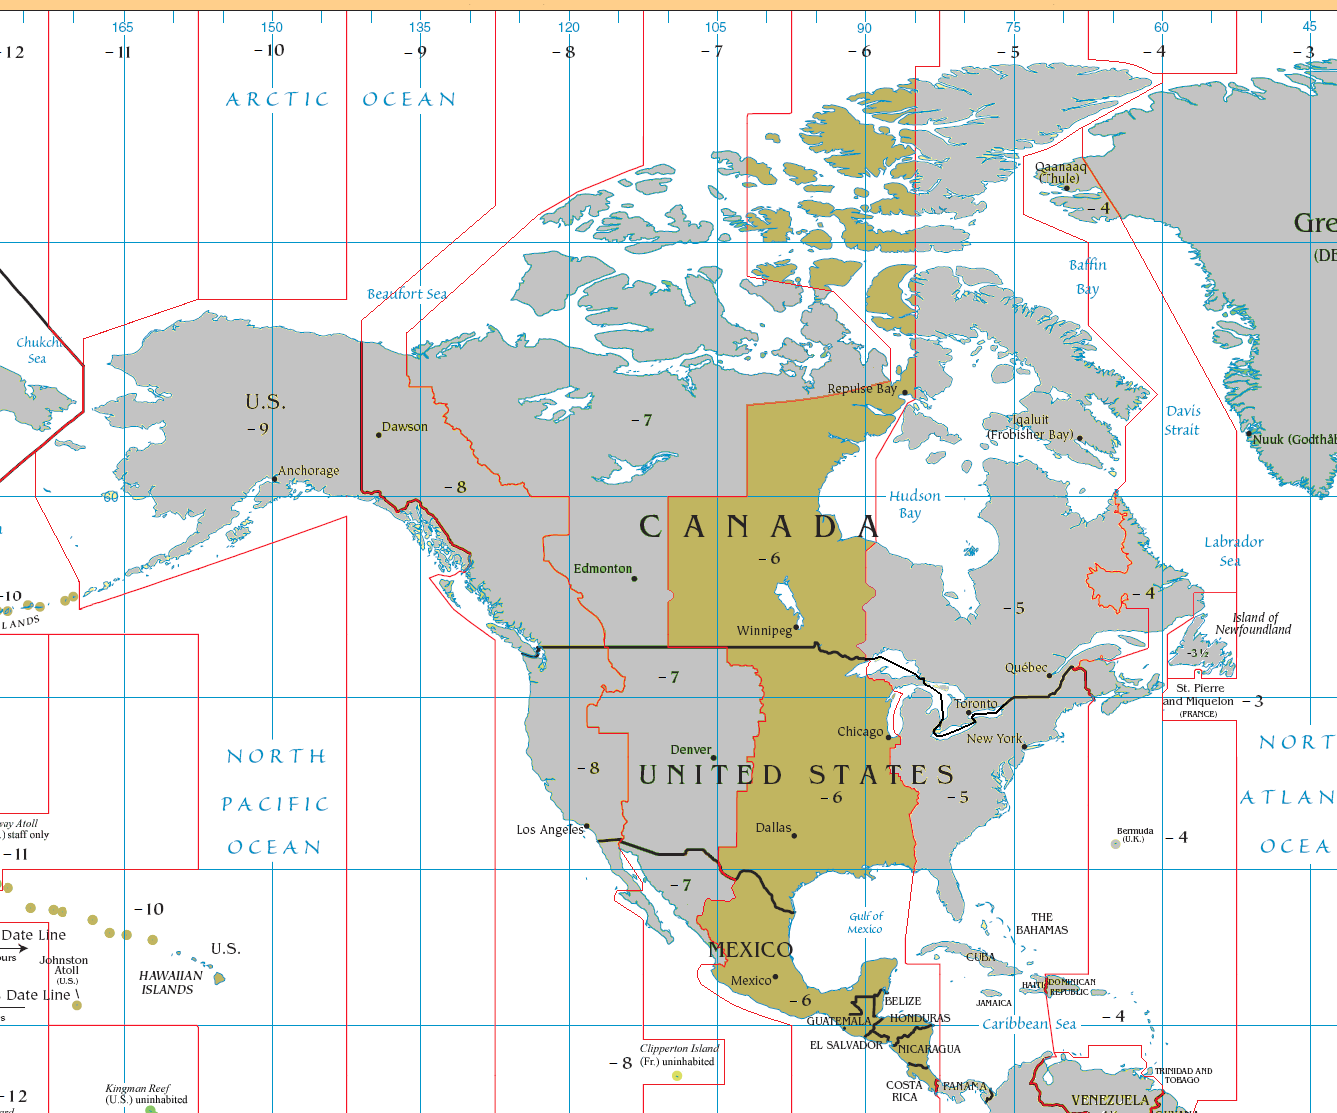
\includegraphics[width=0.5\textwidth]{Husos_horarios.jpg}
\caption{\label{fig:Radación Solar}Huso horario en el Sur de México}
\end{figure}

La imagen anterior nos muestra que el huso horario de la región sur del país es de -6, es decir que hay 6 horas de diferencia entre el sur del pais y del meridiano de Greenwich. 

Entonces si las horas de mayor radiación fueron entre las 17 y 18 horas, en el huso horario de Guerrero el intervalo es de 11-12 de la tarde. 
Posiblemente este detalle del huso horario haya modificado las observaciones de las gráficas anteriores.\\

\textbf{4° ¿Cuál es el lapso de temperatura diaria? (Diferencia entre la temperatura máxima y la mínima).}

Para responder a esta pregunta, consideré el valor máximo de temperatura de todos los datos y el mínimo de todos ellos. La siguiente tabla muestra las diferencias de los máximos y los mínimos de cada magnitud física, entre los cuales la diferencia de temperatura es de 25.8$^{\circ}$ C.\\

\newpage
\begin{figure}[ht!]
\centering
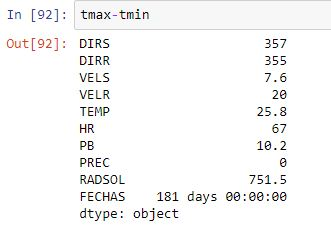
\includegraphics[width=0.5\textwidth]{Diferencia_de_temperaturas.JPG}
\caption{\label{fig:Diferencias de los máximos y mínimos de cada magntiud medida }Diferencias de los máximos y mínimos de cada magntiud medida}
\end{figure} 

\textbf{5°¿Puedes comentar sobre la relación entre la temperatura y la humedad relativa?}

De acuerdo a la gráfica de temperatura y humedad relativa, entre más baja era la temperatura, mayor era la humedad y viceversa, entre más alta la temperatura, menor la humedad.

\begin{figure}[ht!]
\centering
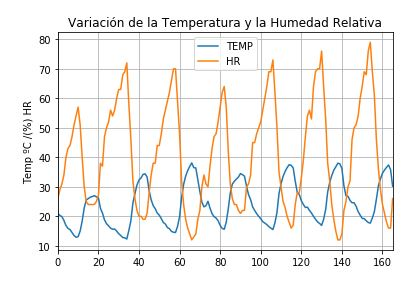
\includegraphics[width=0.5\textwidth]{Variacion_Temp_y_Humedad_Relativa.JPG}
\caption{\label{fig:Diferencias de los máximos y mínimos de cada magntiud medida }Variacion entre la temperatura y la humedad relativa}
\end{figure} 

\textbf{6° Realiza el análisis exploratorio de datos, que resuma el sitio estudiado.}

\begin{figure}[ht!]
\centering
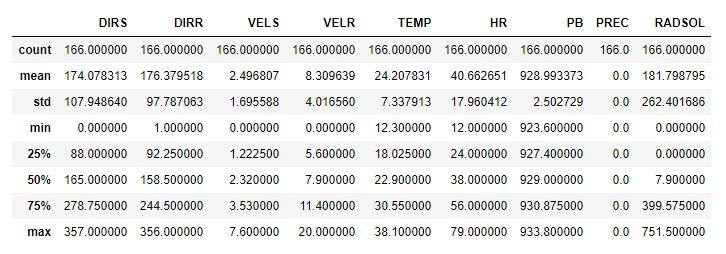
\includegraphics[width=0.5\textwidth]{An_lisis_Exploratorio.JPG}
\caption{\label{fig:Análisis exploratorio de datos }Análisis exploratorio}
\end{figure} 

\section{Conclusión (Apéndice)}
\textbf{1° ¿Cuál es tu primera impresión de Jupyter Notebook?}

Un entorno práctico para programar, ya que en un mismo lugar se pueden hacer gráficas y tablas. 

\textbf{2° ¿Se te dificultó leer código en Python?}

Un poco, tenía nociones básicas, ya que en las vacaciones de invierno empecé a ver un curso en línea sobre introducción a la programación en Python.

\textbf{3° ¿En base a tu experiencia de programación en Fortran, que te parece el entorno de trabajar en Python?}

Siendo un lenguaje de interpretación, te facilita más las cosas al no tener que declarar variables con sus tipos respectivos. 

\textbf{4° A diferencia de Fortran, ahora se producen las gráficas utilizando la biblioteca Matplotlib. ¿Cómo fue tu experiencia?.} 

Tuve un poco de dificultad a la hora de graficar dos listas de datos en una sola gráfica. No obstante, es muy conveniente poder ver en un mismo lugar las gráficas que generas. 

\textbf{5° En general, ¿qué te pareció el entorno de trabajo en Python?}

Pues lo que noté es que está bien estructurado, ya que tiene una gran variedad de librerias especificas para graficar, organizar datos y operar con ellos. 

\textbf{6° ¿Qué opinas de la actividad? ¿Estuvo compleja? ¿Mucho material nuevo? ¿Que le faltó o que le sobró? ¿Qué modificarías para mejorar?}

Bastante material nuevo, considero que se debe de conocer y practicar cada comando y libreria con detalle y tiempo. Considero que debemos comenzar con cuestiones sencillas para aprender Python, tal y como lo hicimos con Fortran, para así ir progresando y subiendo más el nivel de complejidad.

\textbf{7° ¿Comentarios adicionales que desees compartir?}

Tuve dificultades en la parte en la cual se nos pedía obtener las diferencias de temperatura diarias, especificamente en hacer una tabla nueva apartir de una existente con los datos de temperatura y fecha de un intervalo. 


\section{Bibliografía}
\begin{itemize}
  \item Jupyter Features.  Recuperado el 06 de Febrero, 2018, de \url{http://arogozhnikov.github.io/2016/09/10/jupyter-features.html \\}
  \item Why I don't like jupyter fka ipython notebook.  Recuperado el 06 de Febrero, 2018, \url{http://opiateforthemass.es/articles/why-i-dont-like-jupyter-fka-ipython-notebook/}
  \item {\bf Figure 4} recuperado el 07 de Febrero, 2018, de
\url{https://upload.wikimedia.org/wikipedia/commons/d/d7/Central_Time_Zone_CST.png}
\end{itemize} 

\end{document}